\documentclass[crop=false]{standalone}
\usepackage{standard}
\usepackage{eurosym}
\DeclareUnicodeCharacter{20AC}{\text{\euro}}
\usepackage{changepage}
% \usepackage[autostyle,german=guillemets]{csquotes}

\urldef\flogosource\url{http://www.visuallogisticsmanagement.de/wp-content/uploads/2015/10/ITWM.png}
\urldef\slogosource\url{https://www.itwm.fraunhofer.de/en/_jcr_content/stage/stageParsys/stage_slide/image.img.jpg/1498487288072_1440x448-ITWM-beiNacht.jpg}
\urldef\contentsource\url{https://www.itwm.fraunhofer.de/de/ueber-fraunhofer-itwm}

\fancypagestyle{profilestyle}{
  \fancyhf{}
  % \fancyfoot[C]{\footnotesize\bigskip\thepage}
  % \fancyhead[LO,RE]{\footnotesize \thetitle \smallskip} %left
  % \fancyhead[RO,LE]{\footnotesize \theauthor \smallskip} %right
  \renewcommand{\footrulewidth}{0.0pt}
  % \renewcommand{\headrulewidth}{0.5pt}
  \fancyfoot[L]{\rule{150pt}{0.5pt}\\\medskip\footnotesize \hspace{10.5pt} Quellen: \\ \contentsource \\ \flogosource \\ \slogosource}
}

\begin{document}
  \newgeometry{a4paper, lmargin=27mm, rmargin=27mm, tmargin=0mm, bmargin=40mm}
  \thispagestyle{profilestyle}

  \begin{adjustwidth}{-0.4\textwidth}{-0.4\textwidth}
    \center
    \vskip-1em
    {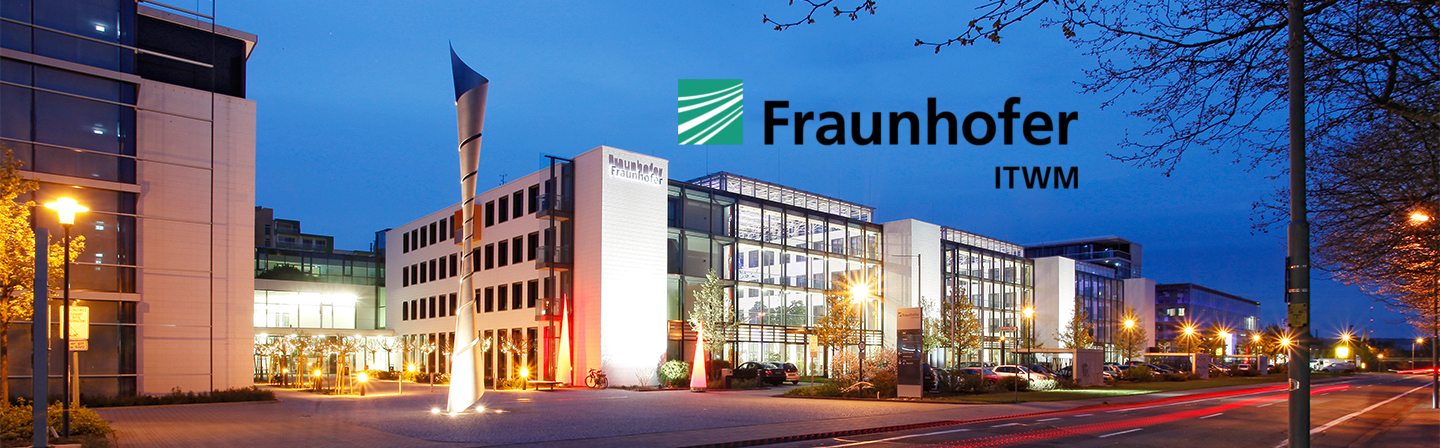
\includegraphics[width=1.65\textwidth]{itwm_logo.jpg}}
  \end{adjustwidth}

  % \bigskip
  \vspace{-1em}

  {\center\tcbox[enhanced,hbox,tikznode,left=8mm,right=8mm,boxrule=0.4pt,
  colback=white,colframe=black!50!white,
  drop lifted shadow=black!50!white,arc is angular,
  before=\par\vspace*{5mm},after=\par\bigskip]{\bf \Large Kurzprofil des Fraunhofer ITWM \\ \bf und der Abteilung CC HPC}}
  \medskip
  \smallskip

  \begin{multicols}{2}
    \parskip=0pt
    \noindent
    Das Fraunhofer ITWM hat seinen Ursprung in dem Institut für Techno- und Wirtschaftsmathematik (ITWM) der Technischen Universität Kaiserslautern, welches am 9.~November 1995 durch die Arbeitsgruppe Technomathematik (AGTM) ins Leben gerufen wurde.
    Das Ziel war die Verbindung von Mathematik und Praxis in Anbetracht von wissenschaftlichem Anspruch und unternehmerischen Denken.
    Am 11.~April 2000 beschloss dann der Senat der Fraunhofer-Gesellschaft die Aufnahme des ITWM zum 1.~Januar 2001.

    Seitdem entwickelt das Fraunhofer ITWM hauptsächlich Simulationssoftware für die Analyse und die Lösung von Problemen im Industriebereich.
    Dabei steht vor allem die mathematische Modellierung verschiedenster realer Prozesse, als auch die Kombination der Hochschulmathematik mit ihrer praktischen Umsetzung im Mittelpunkt.
    Folglich bilden die klassischen Disziplinen der angewandten Mathematik, wie zum Beispiel Numerik, Stochastik oder Optimierung, wichtige Kernkompetenzen des Institutes.
    Beispiele für Geschäftsfelder, auf denen das Fraunhofer \hbox{ITWM} arbeitet, sind Virtuelles Material- und Produktdesign, Prozesssimulation und Diagnosesysteme.
    In jedem dieser Gebiete reichen die angebotenen Produkte von System- und Softwarelösungen bis hin zu Beratungs- und Supportangeboten.

    Seit seiner Gründung ist der Betriebshaushalt des ITWM von anfangs $1.64\appendUnit{Mio.\ €}$ auf $21.5\appendUnit{Mio.\ €}$ im Jahre 2016 angestiegen.
    Inzwischen beschäftigt das Fraunhofer ITWM über 400 Mitarbeiter, die sich von Auszubildenden und wissenschaftlichen Hilfskräften über Doktoranden bis hin zu Arbeitern in den zentralen, wissenschaftlichen und technischen Bereichen erstrecken.
    Die zentrale und moderne IT-Infrastruktur, bestehend aus circa 300 Servern und mehreren Hundert Terabyte Datenspeicher, stellt sowohl Linux- als auch Windows-Architekturen zur Verfügung und bietet den Mitarbeitern damit die  Möglichkeit, effizient auf einer angepassten Umgebung zu forschen.
    Auch resourcenintensive Simulationsrechnungen lassen sich auf dem internen Linux-Hochleistungsrechner \enquote{Beehive} durchführen.
    Das Fraunhofer ITWM gehört damit zur Speerspitze der Mathematik in der Industrie und ist eines der größten und erfolgreichsten Institute der Techno- und Wirtschaftsmathematik.

    Das Competence Center High Performance Computing (CC HPC) ist eine Abteilung des Fraunhofer ITWM, die seit dessen Gründung besteht und sich in enger Zusammenarbeit mit industriellen und akademischen Partnern mit der Frage, wie die immer komplexer werdenden Prozessoren und Parallelrechner effizient genutzt werden können, beschäftigt.
    Sie stellt neben Werkzeugen zum Umgang mit Supercomputern auch komplette Softwarelösungen her und ist eine der tragenden Säulen des Fraunhofer ITWM.
    Insbesondere sind hier die Themenschwerpunkte seismische Datenverarbeitung, photorealistische Visualisierung und skalierbare parallele Programmierung zu nennen.
  \end{multicols}

  \restoregeometry
\end{document}